\chapter{Level 1: Build a network and test its connectivity}

\section{Network Topology}

\begin{figure}[H]
    \centering
    \begin{tikzpicture}[node distance=2.5cm]
    \node (attacker) [draw, circle, fill=red!20, minimum size=2cm] {Attacker 192.168.96.183};
    \node (victim1) [draw, circle, fill=blue!20, minimum size=2cm, below left=of attacker] {Victim 1 192.168.96.110};
    \node (victim2) [draw, circle, fill=blue!20, minimum size=2cm, below right=of attacker] {Victim 2 192.168.109.157};
    \draw [thick] (attacker) -- (victim1);
    \draw [thick] (attacker) -- (victim2);
    \draw [thick] (victim1) -- (victim2);
    \end{tikzpicture}
    \caption{Network Topology}\label{fig:NetworkTopology}
\end{figure}

\section{Connectivity Tests}

The following screenshots demonstrate the successful ICMP ping tests between each machine, confirming that the machines are fully connected, as shown in Figure~\ref{fig:NetworkTopology}. The machines are also fully connected to the internet. We chose to use the \texttt{iperf} tool instead of just browsing, as it reliably generates similar traffic on demand, further enhancing our network's reliability.

\begin{figure}[H]
    \centering
    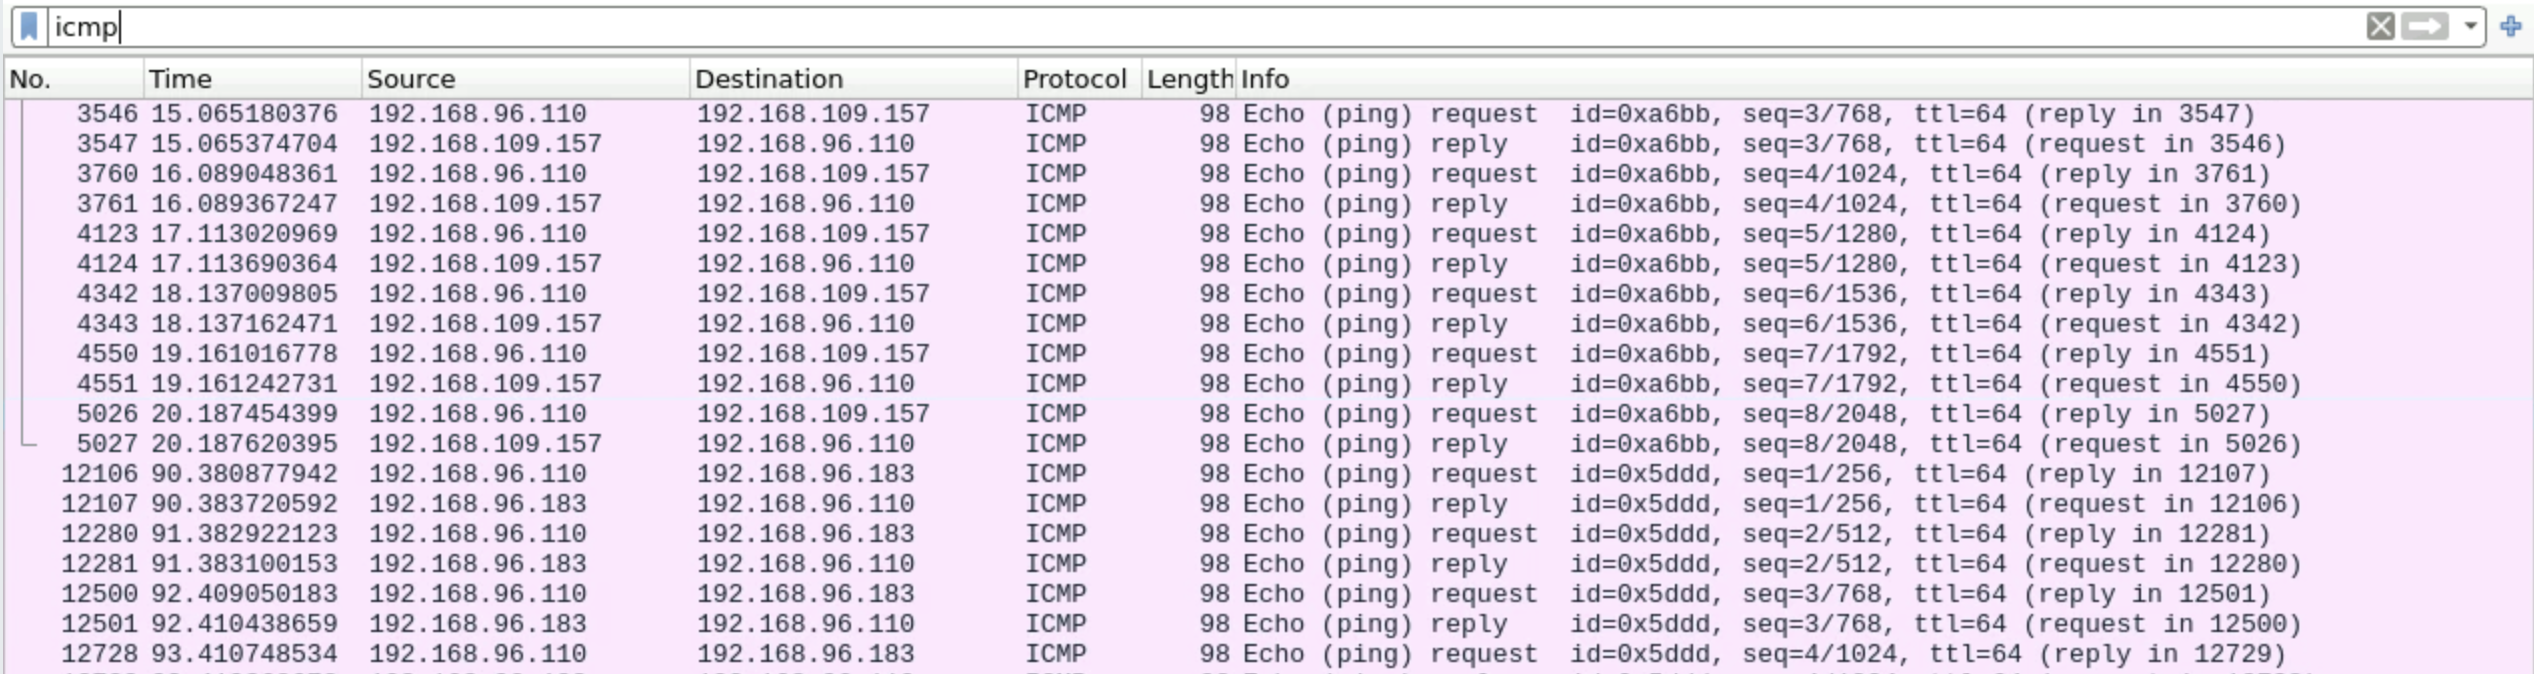
\includegraphics[width=0.8\textwidth]{img/level1/level1-192-168-96-110.png}
    \caption{Pings from Attacker to Other Machines}\label{fig:PingAttacker}
\end{figure}

\begin{figure}[H]
    \centering
    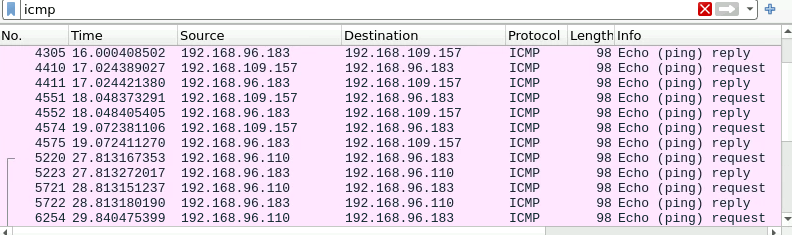
\includegraphics[width=0.8\textwidth]{img/level1/level1-192-168-96-183.png}
    \caption{Pings from Victim 1 to Other Machines}\label{fig:PingVictim1}
\end{figure}

\begin{figure}[H]
    \centering
    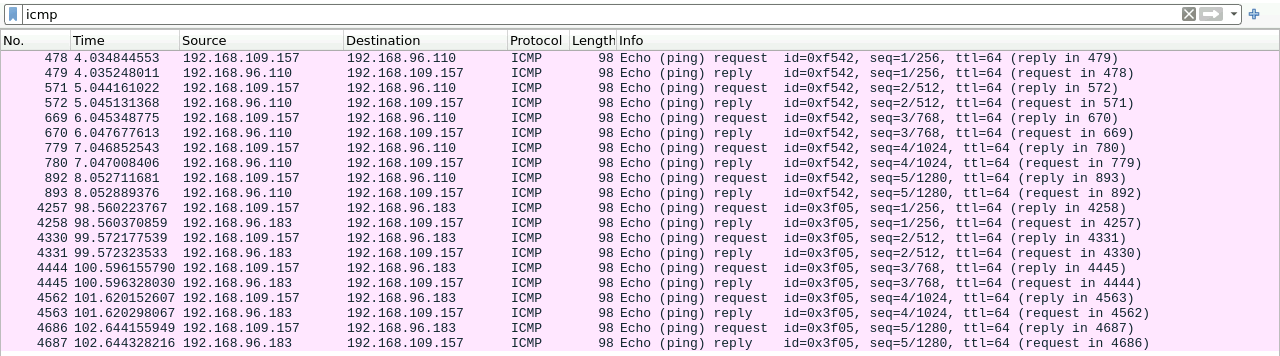
\includegraphics[width=0.8\textwidth]{img/level1/level1-192-168-109-157.png}
    \caption{Pings from Victim 2 to Other Machines}\label{fig:PingVictim2}
\end{figure}